%
%   Dr.HD
%   "robocon.tex"
%

\documentclass[10pt,b5paper,papersize,dvipdfmx]{jsbook}

\usepackage{vuccaken}
\usepackage{vuccaken2019}

% スタイルファイルの読み込みや自作マクロは、
% 最終的には vuccaken2019.sty の中に書いてください。
% とりあえずはここに書いてもらって構いません。


\begin{document} % 以下本文

\setcounter{tocdepth}{2} % 目次にどこまで表示するか
\tableofcontents % 目次出力
\setcounter{page}{0}
\clearpage % 改ページ

% - - - - - - - - - - - - - - - - - - - - - - - - %
\kaishititle%
  {ロボットアーム設計の為の基礎計算}% title
  {ロボティクス学科4回生}% 所属
  {阿部龍幸}% name
% - - - - - - - - - - - - - - - - - - - - - - - - %

\begin{figure}[htbp]
  \centering
  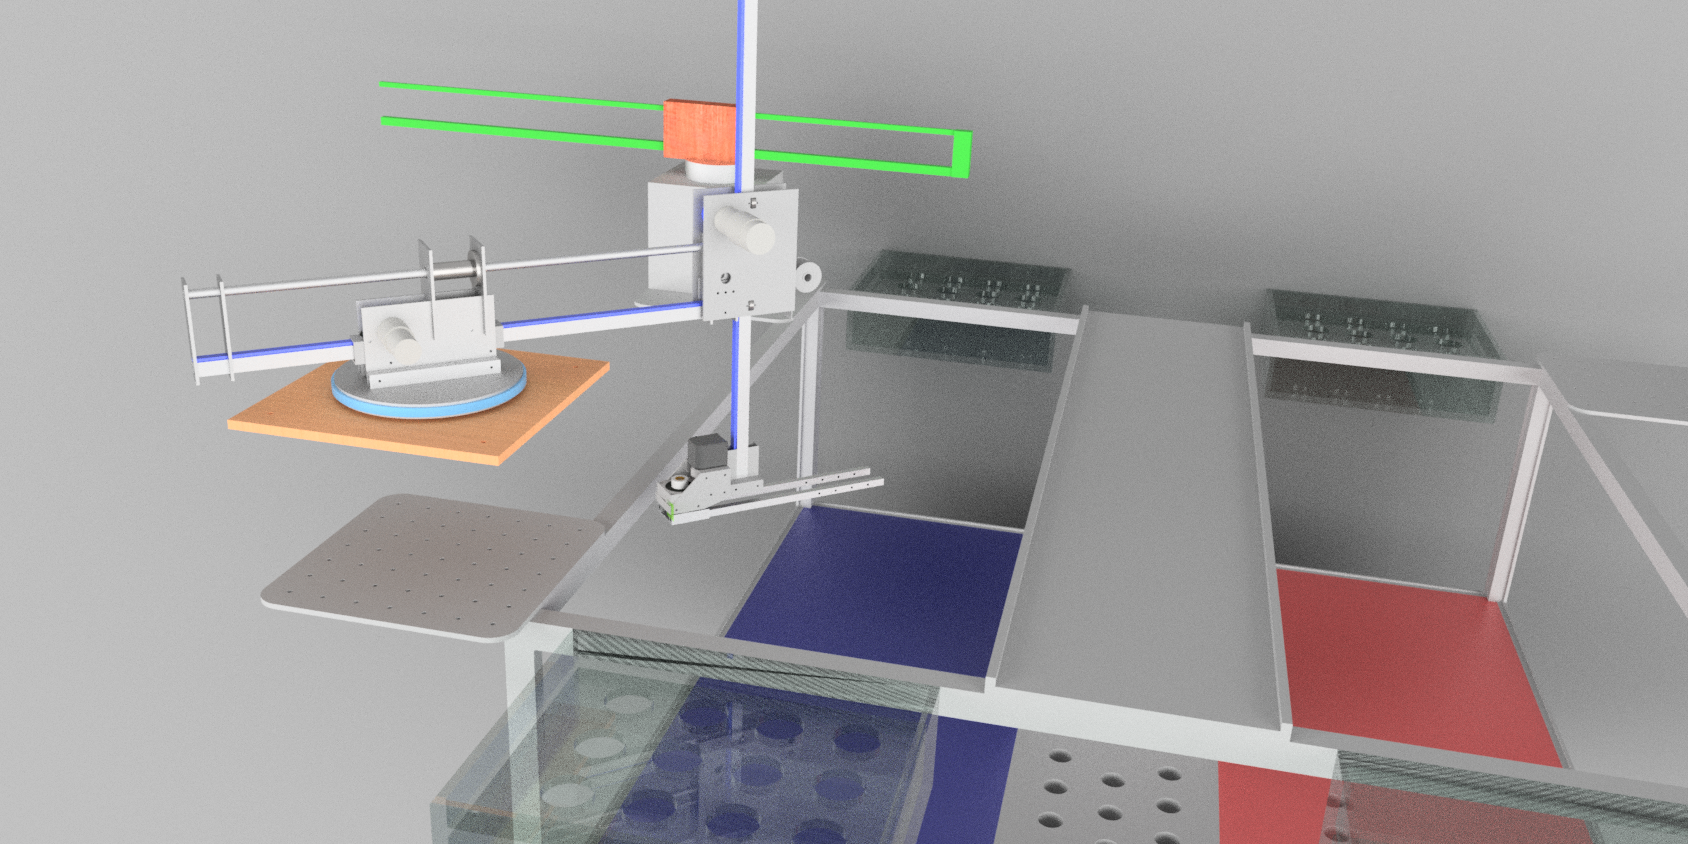
\includegraphics[width=10cm]{robocon/robot_and_field.png}
  % \caption{$y=\sin x$のグラフ。gnuplotで作成した。}
  % \label{fig:robot_and_fields}
\end{figure}

%
\section*{はじめに}
% 会誌ではjsbookクラスを使います。\par
% テーマが複数ある場合は別ファイルで提出してください。
自分が製作予定のロボットアームの最も肝心な一部分の設計をコンピュータによる解析を用いて行う. この設計では, 使用する材質の強度等を考慮しながらアームの形状を変更し, ロボットがユーザの要求する速度を満たすことを目指す. ロボットをCADソフトで設計する際には, 入手可能な材料を以て製作可能な形状を考慮しつつ, 計算に手間のかからない単純な形状を組み合わせたモデルになるように進める. 以下, 物理量をSI単位系で示し, 有効数字を少数点以下2桁とする. 尚, モデルの画像において寸法の表記は[mm]表記とする. 

%
\section{課題設定}
% はじめにこのファイルのソースを自分のtexファイルにコピペしてください。\par
% figureのパスには注意してください。
\subsection{設計目的}
包装されたお菓子などの軽量なワークを素早くハンドリングするロボットアームの, ロボットベースに対して垂直にとった軸周りに素早く回転するアーム部分を設計したい. 回転軸周りのトルク$\tau =1.0 \times 10^3 \tani*{Nm}$ とし, 重力方向の最大変位を $1.0 \times 10^{-2} \tani*{m}$ 以下に抑えることを目指して設計する. また, アームの先には, 実際に製作するロボットが備える機構とハンドを簡略化し, $2.0 \tani*{kg}$ の荷重がかかるパーツを接続する.

%% 参考文献
\begin{sanko}
  \begin{enumerate}
    \item 著者, 本やページの名前, (URL), 出版社, 出版年.
    \item (複数ある場合は追加)
    \item @vuccaken, 物科研HP, \url{rp2017xy.starfree.jp}, 2019.
  \end{enumerate}
\end{sanko}


\end{document}
%
% ファイトだよ!
%
